%%%%%%%%%%%%%%%%%%%%%%%%%%%%%%%%%%%
% Beamer Presentation with UW theme
%%%%%%%%%%%%%%%%%%%%%%%%%%%%%%%%%%%

\documentclass[10pt]{beamer}

\usepackage{siunitx}
\usepackage{tikz}
\usetikzlibrary{shapes.geometric, arrows, chains}
\usepackage[utf8]{inputenc}
\usefonttheme{serif}

\mode<presentation> {
\usetheme[white]{Wisconsin}
%\setbeamertemplate{footline} % To remove the footer line in all slides uncomment this line
%\setbeamertemplate{footline}[page number] % To replace the footer line in all slides with a simple slide count uncomment this line
%\setbeamertemplate{navigation symbols}{} % To remove the navigation symbols from the bottom of all slides uncomment this line
}

\usepackage{graphicx} % Allows including images
\usepackage{booktabs} % Allows the use of \toprule, \midrule and \bottomrule in tables
\usepackage{subfigure}
% Fonts
\setbeamerfont{frametitle}{size={\fontsize{12}{12}},series=\bfseries}
\setbeamerfont{title}{size=\Large,series=\bfseries}
\setbeamertemplate{subsection in toc}[subsections numbered]
\makeatletter
\setbeamertemplate{bibliography item}{\insertbiblabel}
\setbeamertemplate{headline}{%
\leavevmode
\vbox{\begin{beamercolorbox}[dp=1.25ex,ht=4.2ex]{fg=black}%
  \hspace*{1em}\insertsectionhead%
  \ifx\insertsubsectionhead\@empty\relax\else$\quad\mid\quad$\insertsubsectionhead\fi
  \end{beamercolorbox}%
  }%
}
\makeatother

\AtBeginSection[]{
  \begin{frame}
  \vfill
  \centering
  \begin{beamercolorbox}[sep=8pt,center,shadow=true,rounded=true]{title}
    \usebeamerfont{title}\insertsectionhead\par%
  \end{beamercolorbox}
  \vfill
  \end{frame}
}
% Flow Chart
\tikzset{
  process/.style={
    rectangle, 
    %rounded corners,
    minimum width=1cm, 
    minimum height=0.3cm,
    align=center, 
    draw=black, 
    fill=blue!20
    },
  result/.style={
    rectangle, 
    rounded corners,
    minimum width=1cm, 
    minimum height=0.7cm,
    align=center, 
    draw=black, 
    fill=green!20
    },
  arrow/.style={thick,->,>=stealth},
  prod/.style={
    rectangle, 
    rounded corners,
    minimum width=1cm, 
    minimum height=0.7cm,
    align=center, 
    draw=black, 
    fill=white
    },
    pil/.style={
           ->,
           thick,
           shorten <=2pt,
           shorten >=2pt,}
}

%----------------------------------------------------------------------------------------
%	TITLE PAGE
%----------------------------------------------------------------------------------------

\title{Title here}

\author{Moataz S. Harb}
\institute[UWMadison]
{
Department of Engineering Physics \\
\medskip
%\textit{mharb@wisc.edu} % Your email address
}
\date{Month Day, Year}
%
\begin{document}

\begin{frame}
\titlepage
\end{frame}

\begin{frame}
\frametitle{Overview}
\tableofcontents[hideallsubsections]
\end{frame}

%----------------------------------------------------------------------------------------
%	PRESENTATION SLIDES
%----------------------------------------------------------------------------------------

%------------------------------------------------
\section{Section}

\subsection{Subsection}
\begin{frame}
\frametitle{Frame title}
\begin{columns}[c]
\column{.6\textwidth} % Left column and width
\begin{block}{Block}
\begin{itemize}
\item item \cite{paper}
\item item
\begin{equation*}
x + y = z
\end{equation*}
\item fdfdf
\item hghgfd 
\end{itemize}
\end{block}
\begin{block}{block}
\begin{itemize}
\item item 
\begin{itemize}
\item item
\end{itemize}
\end{itemize}
\end{block}
\column{.4\textwidth}
\begin{figure}
\includegraphics[scale=0.06]{figures/joker.jpg}
\caption{figure \cite{paper}}
\end{figure}
\end{columns}
\end{frame}

%------------------------------------------------
\section{section}

\subsection{subsection}
\begin{frame}
\frametitle{title \cite{book}}
\begin{block}{title}
\begin{itemize}
\item item dv d$\hat{\Omega}$ dE in $(\vec{r}, \hat{\Omega}, E)$
\begin{multline*}
  \left[{1 \over v} {\partial \over \partial t} + \hat{\Omega} . \vec{\nabla} + \Sigma(\vec{r}, E)\right]  \psi(\vec{r}, \hat{\Omega}, E, t) = q(\vec{r}, \hat{\Omega}, E, t)
  \\ + \iint dE' d\hat{\Omega'} \Sigma_s(\vec{r}, E' \rightarrow E, \hat{\Omega'} . \hat{\Omega}) \psi(\vec{r}, \hat{\Omega'}, E', t)
\end{multline*}
\begin{itemize}
\item $v$ is 
\end{itemize}
\item item,
\begin{equation*}
  xy=z
\end{equation*}
\end{itemize}
\end{block}
\end{frame}


\begin{frame}
\frametitle{title}
\begin{columns}[T]
\column{.49\textwidth}
\begin{block}{title}
\begin{itemize}
\item item
\end{itemize}
\end{block}
\column{.49\textwidth}
\begin{block}{title}
\begin{itemize}
\item item
\end{itemize}
\end{block}
\end{columns}
\begin{block}{item}
\begin{itemize}
\item item
\end{itemize}
\end{block}
\end{frame}

\subsection{title}
\begin{frame}
\frametitle{title}
\begin{itemize}
\item item
\begin{equation*}
N_1 \rightarrow N_2 \rightarrow ...  \rightarrow N_{n-i} \rightarrow ...  \rightarrow N_{n}
\end{equation*}
\begin{equation*}
  {\partial \over \partial t} N_j(\vec{r}, t) = c
\end{equation*}
\begin{equation*}
  P_{i \rightarrow j} = \lambda_{i \rightarrow j} + \int dE \sigma_{i \rightarrow j}(\vec{r}, E) \phi(\vec{r}, E) 
\end{equation*}
\begin{equation*}
  {\partial \over \partial t}\vec{N}(\vec{r}, t) = \bold{A}\vec{N}(\vec{r}, t)
\end{equation*}
\item item
\end{itemize}
\end{frame}

%------------------------------------------------
\section{section}

\subsection{subsection}

\begin{frame}
\frametitle{title}
\begin{block}{title}
\centering
%\resizebox{!}{.8\textheight}{% if required
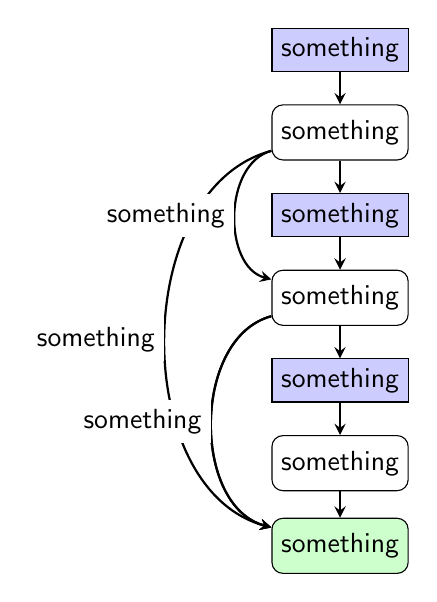
\begin{tikzpicture}
[
  start chain=going below,
  every join/.style={arrow},
  every node/.style={fill=white, font=\sffamily}, align=center],
  node distance=0.4cm
  ]
\node (start) [process,on chain] {something};
\node (node1) [prod,below of=start, yshift=-0.05cm] {something};
\node (node2) [process,below of=node1, yshift=-0.05cm] {something};
\node (node3) [prod,below of=node2, yshift=-0.05cm] {something};
\node (node4) [process,below of=node3, yshift=-0.05cm] {something};
\node (node5) [prod,below of=node4, yshift=-0.05cm] {something};
\node (node6) [result,below of=node5, yshift=-0.05cm] {something};
      
\draw[{arrow}] (start) -- (node1);
\draw[{arrow}] (node1) -- (node2);
\draw[{arrow}] (node2) -- (node3);
\draw[{arrow}] (node3) -- (node4);
\draw[{arrow}] (node4) -- (node5);
\draw[{arrow}] (node5) -- (node6);
\uncover<2>{\draw[bend right=75,{arrow}]  (node1) to node [auto, swap] {something} (node6);}
\uncover<3>{\draw[bend right=75,{arrow}]  (node3) to node [auto, swap] {something} (node6);}
\uncover<4>{\draw[bend right=75,{arrow}]  (node1) to node [auto, swap] {something} (node3);
\draw[bend right=75,{arrow}]  (node3) to node [auto, swap] {something} (node6);}
\end{tikzpicture}%
%}
\end{block}
\end{frame}

%------------------------------------------------
\section{section}
\subsection{subsection}

\begin{frame}
\frametitle{title}
\begin{columns}[T]
\column{.32\textwidth} % Left column and width
\begin{block}{title}
%\resizebox{!}{.8\textheight}{% if required
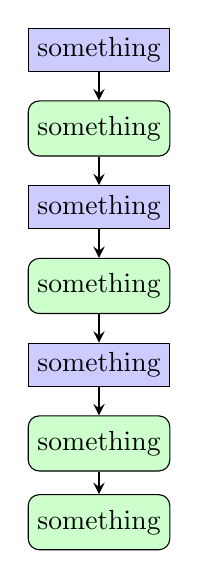
\begin{tikzpicture}[
  start chain=going below,
  every join/.style={arrow},
  node distance=0.4cm
  ]
\node (start) [process,on chain] {something};
\node (node1) [result,below of=start, yshift=-0.6cm] {something};
\node (node2) [process,below of=node1, yshift=-0.6cm] {something};
\node (node3) [result,below of=node2, yshift=-0.6cm] {something};
\node (node4) [process,below of=node3, yshift=-0.6cm] {something};
\node (node5) [result,below of=node4, yshift=-0.6cm] {something};
\node (node6) [result,below of=node5, yshift=-0.6cm] {something};
\draw[{arrow}] (start) -- (node1);
\draw[{arrow}] (node1) -- (node2);
\draw[{arrow}] (node2) -- (node3);
\draw[{arrow}] (node3) -- (node4);
\draw[{arrow}] (node4) -- (node5);
\draw[{arrow}] (node5) -- (node6);
\end{tikzpicture}%
%}
\end{block}
\column{.58\textwidth} % Left column and width
\begin{block}{title}
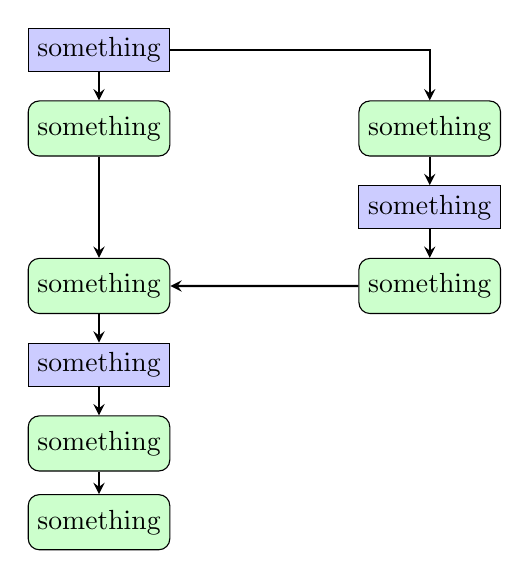
\begin{tikzpicture}[
  start chain=going below,
  every join/.style={arrow},
  node distance=0.4cm
  ]
\node (start) [process,on chain] {something};
\node (node1) [result,below of=start, yshift=-0.6cm] {something};
\node (node2) [result,below of=node1, yshift=-1.6cm] {something};
\node (node3) [process,below of=node2, yshift=-0.6cm] {something};
\node (node4) [result,below of=node3, yshift=-0.6cm] {something};
\node (node5) [result,below of=node4, yshift=-0.6cm] {something};
\node (node6) [result,right of=node1,xshift=3.8cm] {something};
\node (node7) [process,below of=node6, yshift=-0.6cm] {something};
\node (node8) [result,below of=node7, yshift=-0.6cm] {something};
\draw[{arrow}] (start) -- (node1);
\draw[{arrow}] (start) -| (node6);
\draw[{arrow}] (node1) -- (node2);
\draw[{arrow}] (node2) -- (node3);
\draw[{arrow}] (node3) -- (node4);
\draw[{arrow}] (node4) -- (node5);
\draw[{arrow}] (node6) -- (node7);
\draw[{arrow}] (node7) -- (node8);
\draw[{arrow}] (node8) -- (node2);
\end{tikzpicture}%
%}
\end{block}
\end{columns}
\end{frame}

\subsection{subsection}
\begin{frame}
\frametitle{title}
\begin{figure}[ht]
  \centering
  \includegraphics[scale=0.05]{figures/joker.jpg}
\end{figure}
\end{frame}

\begin{frame}
\frametitle{title}
\begin{columns}[c]
\column{.5\textwidth}
\begin{itemize}
\item item
\item item:
\begin{itemize}
\item item
\end{itemize}
\end{itemize}
\column{.6\textwidth}
\begin{figure}[ht]
\includegraphics[scale=0.08]{figures/joker.jpg}
\end{figure}
\end{columns}
\end{frame}

%------------------------------------------------
\section{}
\begin{frame}
\vfill
\centering
\begin{beamercolorbox}[sep=8pt,center,shadow=true,rounded=true]{title}
  \usebeamerfont{title}{THANK YOU}
\end{beamercolorbox}
\vfill
\end{frame}

%------------------------------------------------
\section{References}
\begin{frame}[allowframebreaks=1]
\frametitle{References}
\small
\bibliographystyle{unsrtnat}
\begin{thebibliography}{0.2}
\bibitem{paper}
{title, journal, vol. number (year)}
\bibitem{book}
authors, {title, publisher (year)}
\end{thebibliography}
\end{frame}

\end{document} 